\section{Aufgaben (TiK)}
Wesentliche Fragestellungen, die in diesem Kapitel gelöst werden sollen, sind auf der einen Seite, herauszufinden, welche vorhandenen IT-Systeme bereits zentral Verwendung finden und auf der anderen Seite, wie Informationen aktuell repräsentiert werden. Des weiteren soll in dieser Analyse Aufschluss darüber gegeben werden, ob ein Informationsmanagement an der Hochschule betrieben wird und wie Informationen bereits zentral zur Verfügung gestellt werden.

Die Hochschule Emden/Leer ist eine kleine Hochschule mit aktuell 4626 eingeschriebenen Studierenden. Den größten Anteil machen die 4303 Studenten vor Ort aus.\footnote{\url{http://www.hs-emden-leer.de/fileadmin/user_upload/Einrichtungen/ZDF/Studierende/JV_Stud_20142.pdf}} Es sind 396 Mitarbeiter beschäftigt, wobei 107 Professuren sind.\footnote{\url{https://www.hs-emden-leer.de/no_cache/hochschule/zahlen-daten-fakten.html}}

Ein Hauptbestandteil dieses Kapitels ist der Prozess der Sammlung, Selektion und Prüfung von Fragestellungen, die die Grundlage für ein Experteninterview bilden. Im Rahmen dieser Ausarbeitung wurde sich für die Verwendung eines Experteninterviews entschieden, da hier die Zielgruppe ein Spezialist ist. In diesem Fall ist der Interviewte der Leiter des Hochschulrechenzentrums der Hochschule Emden/Leer, Herr Günter Müller. Das Experteninterview führten die Studierenden Tina Koppermann, Marc Enders, die betreuende Professorin Frau Prof. Dr. Krüger-Basener mit Herrn Günter Müller durch. 

Bei der Erstellung des Experteninterviews wurde auf die Methodik des SPSS-Prinzipes verstärkt reflektiert. Dem SPSS-Prinzip nach Helfferich\footnote{\cite{helfferich_2009}} liegt folgendes Vorgehen zur Grunde:

\begin{enumerate}
	\item Sammeln
	\item Prüfen
	\item Selektieren
	\item Subsumieren		
\end{enumerate}

Mit Hilfe des Prinzips zur qualitativen Datenerhebung fand im ersten Schritt das Sammeln von Fragen statt. Diese konnten von allen Kursteilnehmern in einem zur Verfügung gestellten Online-Dokument eingesehen und editiert werden. Bei der Sammlung der Fragen sind insgesamt 62 Fragestellungen zu unterschiedlichen Schwerpunkten aufgenommen worden (siehe Abbildung \ref{fig_auszug_fragen_sammeln}).

\begin{figure}[h!]
	\centering
	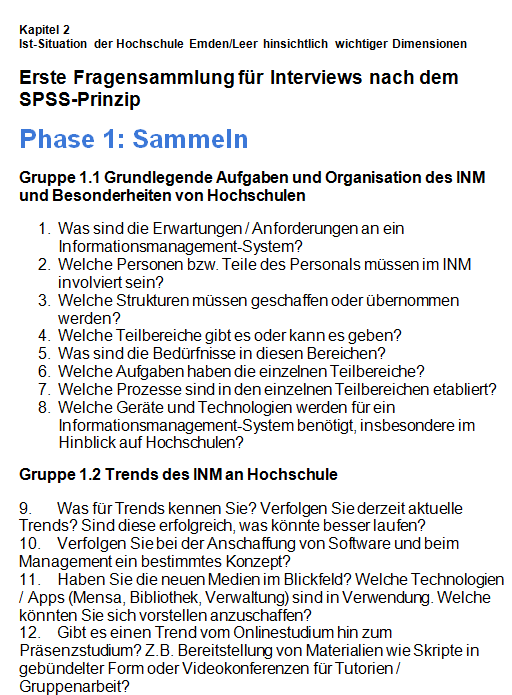
\includegraphics[width=10cm]{kapitel/gruppe2/bilder/auszug_fragen}
	\caption{Auszug der gesammelten Fragen}
	\label{fig_auszug_fragen_sammeln}
\end{figure}

Nach Abschluss der Sammlung aller Fragen, folgte im zweiten Schritt die Prüfung dieser. Hierbei wurden reine Informationsfragen direkt aussortiert. 

Im darauffolgenden Schritt erfolgte die Selektion der Fragen, indem entsprechend nach Themengebieten kategorisiert wurde. 

Beim Subsumieren wurde für jede Thematik eine Erzählaufforderung gefunden und die Gliederung des Interviewfadens entsprechend erstellt. Wie in Abbildung \ref{fig_farbcode_SPSS} dargestellt erfolgte mit Hilfe eines Farbcodes die farbliche Markierung und Einsortierung der Fragen entsprechend nach Erzählaufforderung, Checkliste, konkreter Frage und Aufrechterhaltungsfrage. Ein Auszug der visuell farblich aufbereiteten Subsumtion ist in Abbildung \ref{fig_sortierung_fragentyp} zu sehen.

\begin{figure}[h!]
	\centering
	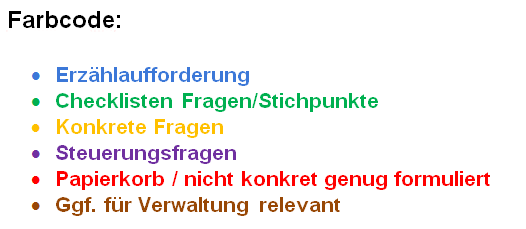
\includegraphics[width=10cm]{kapitel/gruppe2/bilder/farbcode_spss}
	\caption{angewandter Farbcode für das SPSS-Prinzip}
	\label{fig_farbcode_SPSS}
\end{figure}

\begin{figure}[h!]
	\centering
	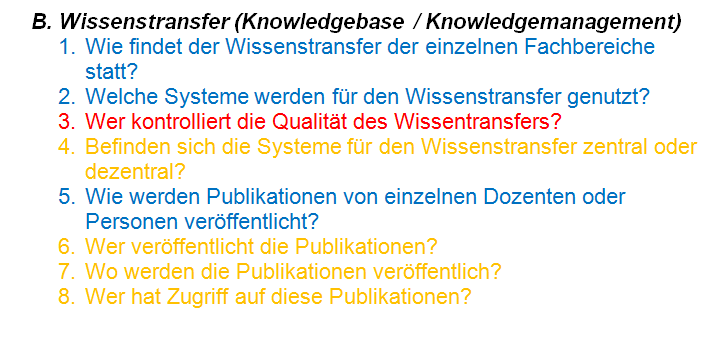
\includegraphics[width=10cm]{kapitel/gruppe2/bilder/sortierung_fragentyp}
	\caption{Sortierung der Fragen nach Fragentyp}
	\label{fig_sortierung_fragentyp}
\end{figure}

Die Visualisierung der Subsumtion fand mit Hilfe des Anwendungsprogramms Microsoft Excel statt. Als Endergebnis ist ein in acht unterschiedliche Themenbereiche gegliederter Interviewleitfaden entstanden (siehe Abbildung: \ref{fig_auszug_interviewleitfaden}).

\begin{figure}[h!]
	\centering
	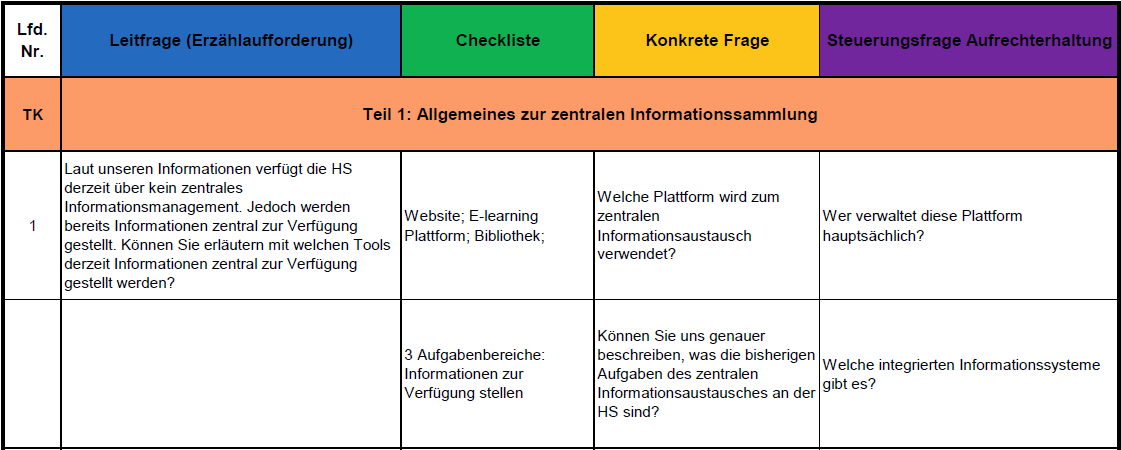
\includegraphics[width=10cm]{kapitel/gruppe2/bilder/auszug_leitfaden}
	\caption{Auszug des Interviewleitfadens}
	\label{fig_auszug_interviewleitfaden}
\end{figure}

An einem festgelegtem Interviewtermin ist mit Hilfe dieses Leitfadens das Experteninterview mit Herrn Günter Müller durchgeführt worden. Für die Durchführung des Interviews wurde die Online Video Plattform „Adobe Connect“ genutzt. Herr Müller stimmte der digitalen Aufzeichnung zu. Im Anschluss an das Experteninterview erfolgte in der ersten Phase die Analyse der Aufzeichnung auf wichtige inhaltliche Aspekte.

Wie in Abbildung \ref{fig_E-Learning_Transkription} exemplarisch zu sehen ist, wurde in der zweiten Phase durch Transkription die zur Verfügung gestellte Aufzeichnung mit Hilfe der Applikation „Microsoft Word“ überführt, um die im Interview erhaltenen Informationen besser verarbeiten zu können.

\begin{figure}[h!]
	\centering
	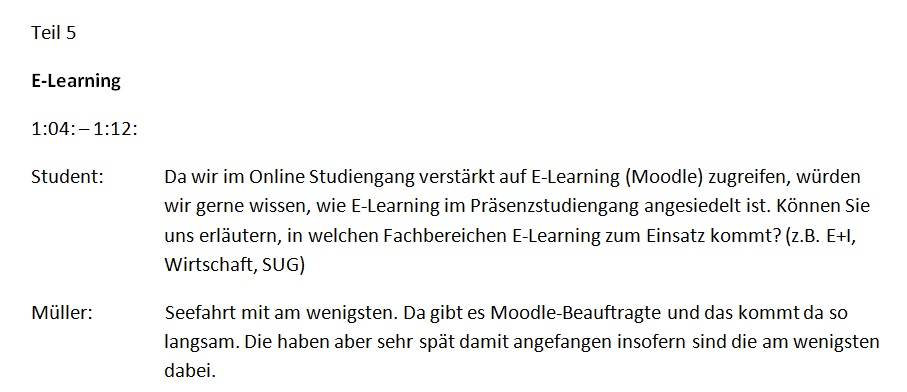
\includegraphics[width=10cm]{kapitel/gruppe2/bilder/E-Learning_Transkription}
	\caption{Transkription: E-Learning}
	\label{fig_E-Learning_Transkription}
\end{figure}

In der dritten und letzten Phase wurde mit Hilfe des Tools „XMind6“ zu jedem Themenbereich ein entsprechendes Mindmap generiert, um somit bei der Recherche schneller auf Besonderheiten eingehen zu können  (siehe Abbildung \ref{fig_E-Learning_MM}).

\begin{figure}[h!]
	\centering
	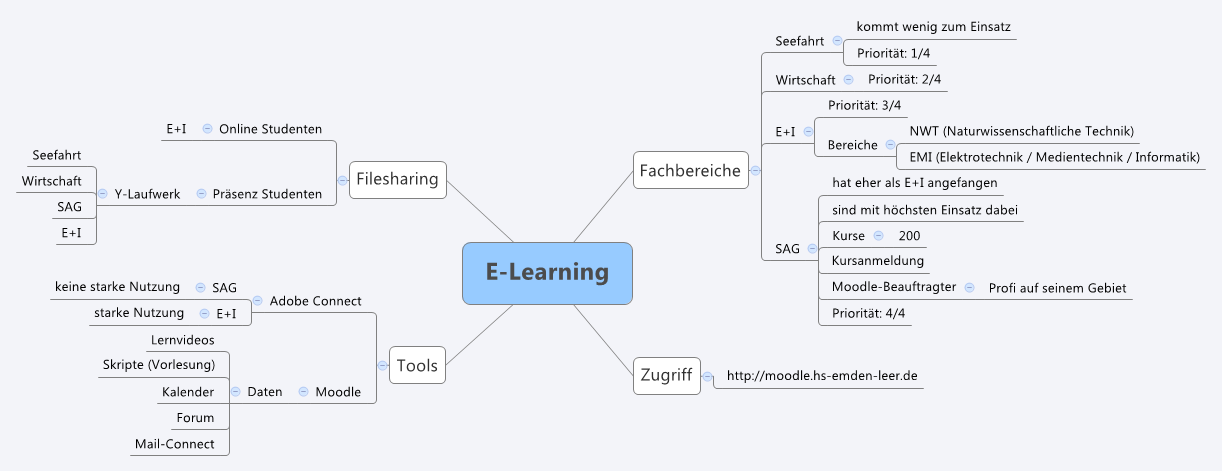
\includegraphics[width=10cm]{kapitel/gruppe2/bilder/E-Learning_MM}
	\caption{Mindmap: E-Learning}
	\label{fig_E-Learning_MM}
\end{figure}

Die Ergebnisse dieser Analyse werden in den folgenden Kapiteln detaillierter beschrieben. 
